\documentclass[letterpaper,12pt]{article}
\usepackage{array}
\usepackage{threeparttable}
\usepackage{geometry}
\usepackage{float}
\geometry{letterpaper,tmargin=1in,bmargin=1in,lmargin=1.25in,rmargin=1.25in}
\usepackage{fancyhdr,lastpage}
\pagestyle{fancy}
\lhead{}
\chead{}
\rhead{}
\lfoot{}
\cfoot{}
\rfoot{\footnotesize\textsl{Page \thepage\ of \pageref{LastPage}}}
\renewcommand\headrulewidth{0pt}
\renewcommand\footrulewidth{0pt}
\usepackage[format=hang,font=normalsize,labelfont=bf]{caption}
\usepackage{listings}
\lstset{frame=single,
  language=Python,
  showstringspaces=false,
  columns=flexible,
  basicstyle={\small\ttfamily},
  numbers=none,
  breaklines=true,
  breakatwhitespace=true
  tabsize=3
}
\usepackage{amsmath}
\usepackage{amssymb}
\usepackage{amsthm}
\usepackage{harvard}
\usepackage{setspace}
\usepackage{float,color}
\usepackage[pdftex]{graphicx}
\usepackage{hyperref}
\hypersetup{colorlinks,linkcolor=red,urlcolor=blue}
\theoremstyle{definition}
\newtheorem{theorem}{Theorem}
\newtheorem{acknowledgement}[theorem]{Acknowledgement}
\newtheorem{algorithm}[theorem]{Algorithm}
\newtheorem{axiom}[theorem]{Axiom}
\newtheorem{case}[theorem]{Case}
\newtheorem{claim}[theorem]{Claim}
\newtheorem{conclusion}[theorem]{Conclusion}
\newtheorem{condition}[theorem]{Condition}
\newtheorem{conjecture}[theorem]{Conjecture}
\newtheorem{corollary}[theorem]{Corollary}
\newtheorem{criterion}[theorem]{Criterion}
\newtheorem{definition}[theorem]{Definition}
\newtheorem{derivation}{Derivation} % Number derivations on their own
\newtheorem{example}[theorem]{Example}
\newtheorem{exercise}[theorem]{Exercise}
\newtheorem{lemma}[theorem]{Lemma}
\newtheorem{notation}[theorem]{Notation}
\newtheorem{problem}[theorem]{Problem}
\newtheorem{proposition}{Proposition} % Number propositions on their own
\newtheorem{remark}[theorem]{Remark}
\newtheorem{solution}[theorem]{Solution}
\newtheorem{summary}[theorem]{Summary}
%\numberwithin{equation}{section}
\bibliographystyle{aer}
\newcommand\ve{\varepsilon}
\newcommand\boldline{\arrayrulewidth{1pt}\hline}
\graphicspath{{images/}}


\begin{document}

\begin{flushleft}
  \textbf{\large{Problem Set \#2}} \\
  MACS 30100, Dr. Evans \\
  Ningyin Xu
\end{flushleft}

\vspace{5mm}

\noindent\textbf{Problem 1. Some income data, lognormal distribution, and hypothesis testing.}\\

\noindent\textbf{Part (a).} \\
\begin{figure}[htb]\centering\captionsetup{width=4.0in}
  \label{Fig1a}
  \fbox{\resizebox{4.0in}{3.0in}{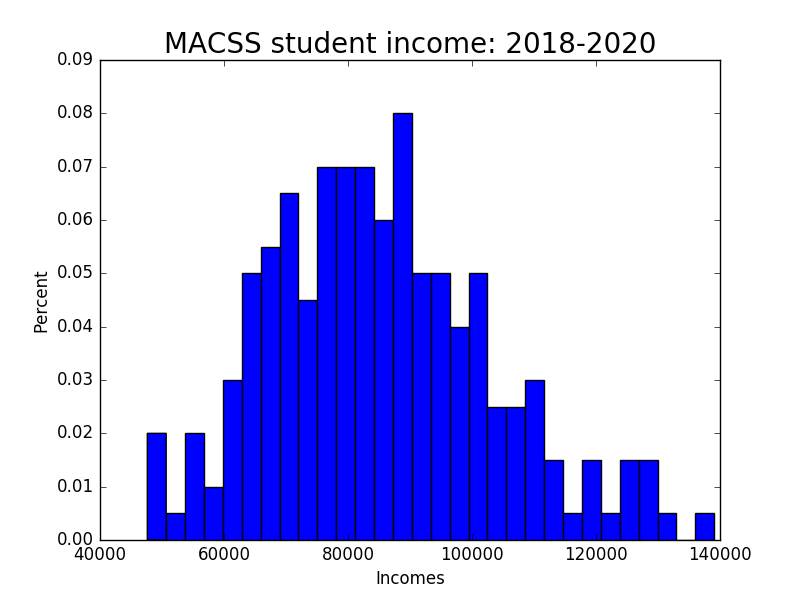
\includegraphics{Fig_1a.png}}}
\end{figure}\\
\\

\noindent\textbf{Part (b).} 
\\
The value of the log likelihood value for this parameterization of the distribution
and given this data is $-8298.64$.\\

\noindent\textbf{Part (c).}
\\
Firstly, $\mu_{mle}=11.331,\sigma_{mle}=0.212$. \\
\\
The log likelihood value of the data given these parameters is $-2239.53$.\\
\\
The variance-covariance matrix is:
$
\begin{bmatrix} 
0.00023979 & 0.00000351\\ 
0.00000351 & 0.00011245\\ 
\end{bmatrix}
$
\\

\newpage
\begin{figure}[htb]\centering\captionsetup{width=4.0in}
  \label{Fig1b}
  \fbox{\resizebox{4.0in}{3.0in}{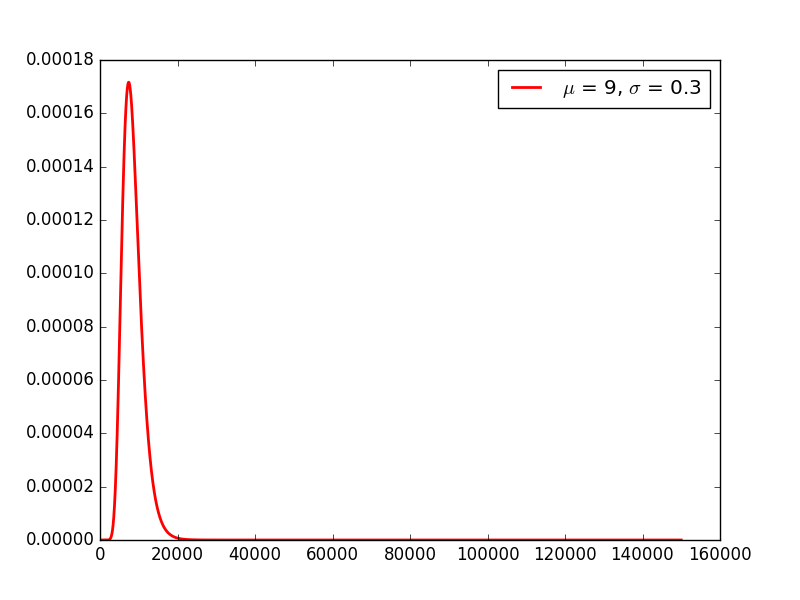
\includegraphics{Fig_1b.png}}}
\end{figure}
\begin{figure}[htb]\centering\captionsetup{width=4.0in}
  \label{Fig1c}
  \fbox{\resizebox{4.0in}{3.0in}{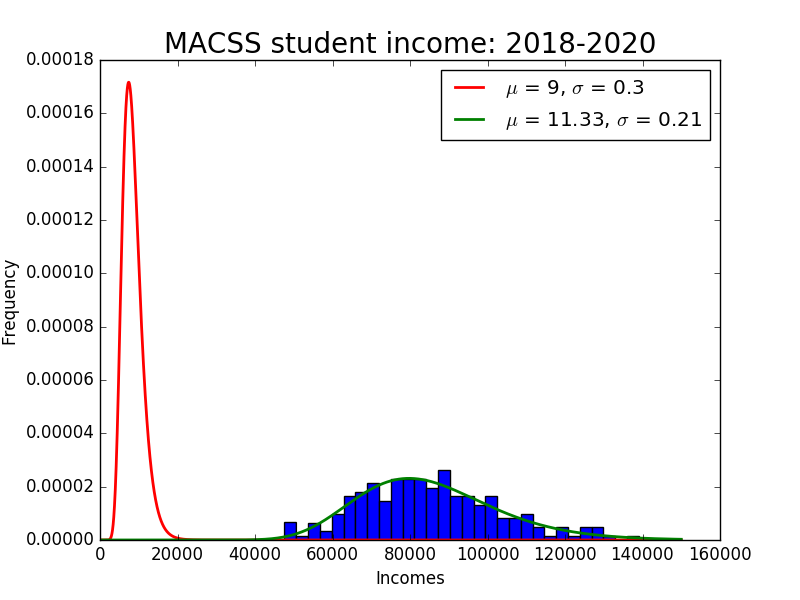
\includegraphics{Fig_1c.png}}}
\end{figure}

\noindent\textbf{Part (d).}
The Chi square of H0 with 2 degrees of freedom p-value = $0.00000000$. Since this probability is small ($< 0.05$), the data is unlikely coming from the distribution in part(b).\\

\noindent\textbf{Part (e).}
The probability that a student would earn more than \$100,000 is: $19.56\%$.\\
The probability of a student earn less than \$75,000 is: $30.79\%$.\\

\newpage

\noindent\textbf{Problem 2. Linear regression and MLE.}\\
\\
\noindent\textbf{Part (a).}\\
\\
$\beta^{mle}_{0} = .252\quad \beta^{mle}_{1} = 0.013\quad\beta^{mle}_{2} = 0.401\quad \beta^{mle}_{3} = -0.009992\quad\sigma^{2}_{mle}=0.00000911$
\\
The value of the log likelihood function is: $876.87$.
\\
\\
The variance-covariance matrix is:
$
\begin{bmatrix}
 1&  0&  0&  0&0 \\ 
 0&  1&  0&  0&0 \\ 
 0&  0&  1&  0&0 \\ 
 0&  0&  0&  1&0 \\ 
 0&  0&  0&  0&1
\end{bmatrix}
$
\\
\\
\noindent\textbf{Part (b).}
\\
Likelihood Ratio Test p-value is: 0.00000000.\\
\\
This number is really low ($< .05$), so it is unlikely that age, number of children, and average winter temperature have no effect onthe number of sick days.\\

\end{document}










